
\section{仿真测试}

\subsection{Hamming 编解码}



\subsection{交织与解交织}



\subsection{QPSK 调制解调}



\subsection{AWGN 信道模型}

我们保存了仿真产生的高斯白噪声数值,并进行了正态分布假设检验

\begin{codeblock}{verilog}
integer log_file;
initial log_file = $fopen("simulation_log.txt", "w");
always @(posedge clk) begin
    $fwrite(log_file, "%d\n", gaussian_noise_channel_0.gaussian_o_0);
    $fflush(log_file);
end
\end{codeblock}

得到高斯白噪声序列(1000 条),并进行正态分布检验,结果如图 \ref{fig:gaussian_simulation} 所示。可见,概率密度分布和 QQ 图均符合高斯分布的特性。


下面进行严格的正态性检验:

首先进行 Shapiro-Wilk 正态性检验,得到统计量 $W = 0.998$,$p = 0.310$,因此我们无法拒绝高斯分布的假设;同时进行 Kolmogorov-Smirnov 正态性检验,得到统计量 $D = 0.027$,$p = 0.462$,同样无法拒绝高斯分布的假设。

\begin{figure}[ht]
    \centering
    \begin{subfigure}[b]{0.48\textwidth}
        \centering
        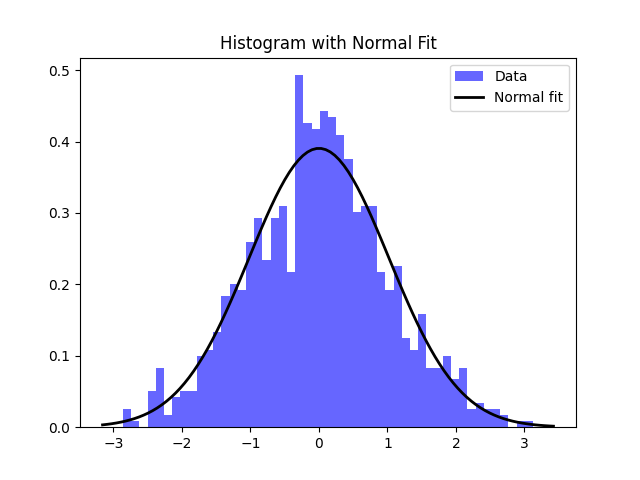
\includegraphics[width=\textwidth]{static/gaussian_fit.png}
        \caption{
            高斯白噪声概率密度分布可视化
        }\label{fig:gaussian_fit}
    \end{subfigure}
    \hfill
    \begin{subfigure}[b]{0.48\textwidth}
        \centering
        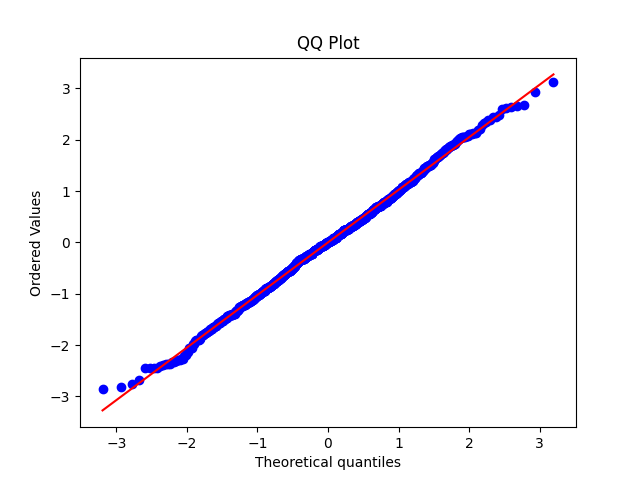
\includegraphics[width=\textwidth]{static/gaussian_qq.png}
        \caption{
            高斯白噪声 QQ 图
        }\label{fig:gaussian_qq}
    \end{subfigure}
    \caption{
        高斯白噪声分布检验
    }\label{fig:gaussian_simulation}
\end{figure}

最后检验自相关性,如图 \ref{fig:gaussian_acf} 所示,分别取 lag 为 40 和 100,自相关性函数均在 0 附近波动,且绝大部分位于 95\% 置信区间内,因此我们可以认为噪声序列是独立同分布的。


\begin{figure}[ht]
    \centering
    \begin{subfigure}[b]{0.48\textwidth}
        \centering
        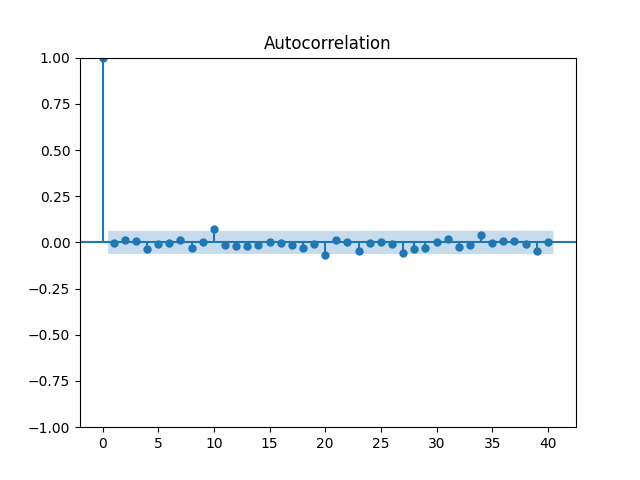
\includegraphics[width=\textwidth]{static/gaussian_acf_40.png}
        \caption{
            高斯白噪声 ACF(lag=40)
        }\label{fig:gaussian_acf_40}
    \end{subfigure}
    \hfill
    \begin{subfigure}[b]{0.48\textwidth}
        \centering
        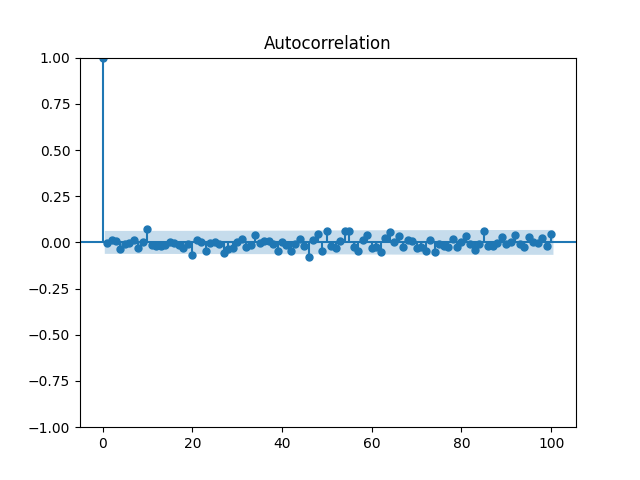
\includegraphics[width=\textwidth]{static/gaussian_acf_100.png}
        \caption{
            高斯白噪声 ACF(lag=100)
        }\label{fig:gaussian_acf_100}
    \end{subfigure}
    \caption{
        高斯白噪声自相关性检验
    }\label{fig:gaussian_acf}
\end{figure}